\documentclass[12pt]{article}
\usepackage[utf8]{inputenc}
\usepackage{amsmath}
\usepackage[T1]{fontenc}

\title{ECE 3413 Lab 05\\*Time Response of First-\\*and Second-Order Systems}
\author{Leomar Dur\'an}
\date{${06}^{\text{th}}$ March 2023}

\usepackage{hyperref}

\usepackage{cancel}
\usepackage[per-mode=symbol]{siunitx}
\newcommand*\siexpr[2][]{\SI[parse-numbers=false,#1]{#2}}%
\usepackage{xfrac}
\usepackage{amssymb}
\newcommand*\transpose{\mathsf{T}}

\usepackage{mathtools}%
\DeclarePairedDelimiter\brao()%
\DeclarePairedDelimiter\brac[]%
\DeclarePairedDelimiter\braco[)%
\DeclarePairedDelimiter\Brac\{\}%
\DeclarePairedDelimiter\abs||
\DeclarePairedDelimiter\norm\lVert\rVert%
\DeclarePairedDelimiter\piecefn\{.
\DeclarePairedDelimiter\evalat.|

\usepackage{lib/nonfloatenvirons}
\usepackage{booktabs}
\newcommand\ra[1]{\renewcommand*\arraystretch{#1}}
\ra{1.25}
\usepackage{minted}

\usepackage{adjustbox}
\newcommand*\mcadj[7]%
% {#columns}{col spec}{rotation}{adjust spec}
% {before rotated text}{rotated text}{after rotated text}
{%
    \multicolumn{#1}{#2}{%
        \rlap{%
            #5\adjustbox{rotate=#3,#4}{#6}~#7%
        }%
    }%
}

\usepackage{pdfpages}
\usepackage{standalone}
\usepackage{matlab}

\usepackage[skip=\baselineskip,indent=0pt]{parskip}
\setlength\parindent{0pt}

\def\hr{{\par\noindent\rule{\textwidth}{0.4pt}}}

\begin{document}

\maketitle
\newpage

\section{Introduction}

The purpose of this experiment is to apply the concept of transfer functions to a translational mechanical system.

The principles used in electrical engineering are shared with other disciplines of engineering.
We can apply these principles to help us look at everyday problems such as a translational system differently,
or we can use this familiarity to better understand the effect of a transfer function in a control system.

This lab also introduces a new type of transfer function, the state-space model which is represented by the \mintinline{matlab}{ss} class in Matlab.

\section{Procedure}

\subsection{Task 1 -- The effect of poles and natural frequency}

\begin{enumerate}
    \item
        Given the transfer function
        \begin{equation}
            G_2\brao*s = \frac{b}{s^2 + as + b},
        \end{equation}
        
        let the damping ratio and natural frequency, respectively $\zeta, \omega_n \in \mathbb{R}$ s.t. $a = 2\zeta\omega_n$ and $b = \omega_n^2$. So
        \begin{equation}
            \piecefn*{
                \begin{matrix}
                    \omega = \sqrt{b}\rlap, \\*
                    \zeta = \dfrac{a}{2\sqrt{b}}\rlap. \\*
                \end{matrix}
            }\rlap{$\qquad\brao*{b > 0}$}
        \end{equation}

        Furthermore
        \begin{equation}
            \zeta\omega_n = \frac{a}2,
        \end{equation}
        and
        \begin{equation}
            \sqrt{1 - \zeta^2} = \sqrt{1 - \brao*{\sfrac{a}{\brao*{2\sqrt{b}}}}^2} = \frac{1}{2\sqrt{b}} \sqrt{4b - a^2}.%
            \hskip1em\brao*{\abs*{a} \leq 2\sqrt{b}}
        \end{equation}
        
        We find that the peak time
        \begin{equation}
            T_p = \frac\pi{\omega_n \sqrt{1 - \zeta^2}} = \frac\pi{\brao*{\sqrt{b}}\brao*{ \frac{1}{2\sqrt{b}}\sqrt{4b - a^2}}} = \frac{2\pi}{\sqrt{4b - a^2}}.
        \end{equation}

        We find that the overshoot rate
        \begin{equation}
            \begin{array}{*2{@{}r}@{}l@{}}
                \% OS
                &{}:={}& \exp\brao*{\dfrac{-\zeta\pi}{\sqrt{1 - \zeta^2}}} \SI{100}\percent
            \\*[1.3em]
                &{}={}& \exp\brao*{-\zeta\omega_n\brao*{\dfrac{\pi}{\omega_n\sqrt{1 - \zeta^2}}}} \SI{100}\percent
            \\*
                &{}={}& \exp\brao*{-\brao*{\zeta\omega_n}^{\vphantom{1}}T_p} \SI{100}\percent
            \\*
                &{}={}& \exp\brao*{-\brao*{\tfrac{a}2}^{\vphantom{1}}T_p} \SI{100}\percent
            \\*
                & {}={} & \exp\brao*{\dfrac{-aT_p}{2}} \SI{100}\percent\rlap.
            \\*
            \end{array}
        \end{equation}

        We find that the settling time
        \begin{equation}
            T_s \approx \frac4{\zeta\omega_n} = \frac4{\brao*{\sfrac{a}2}} = \frac8a.
        \end{equation}

        To find rise time, we must first find the step response in the time domain with parameters substituted.

        \subsubsection{Step response}
        We have
        \[
            G_2\brao*s = \frac{b}{s^2 + as + b},
        \]

        Well
        \begin{equation}
            C\brao*s = R\brao*s G_2\brao*s = \frac1s \frac{b}{s^2 + as + b}.
        \end{equation}

        So the second order factor of the denominator
        \begin{equation}
            \begin{aligned}
                s^2 + as + b
                &{} = \brao*{s^2 + 2\brao*{\frac{a}2}s + \brao*{\frac{a}2}^2} + \brao*{b - \brao*{\frac{a}2}^2}
            \\*
                &{} = \brao*{s + \frac{a}2}^2 + \brao*{\sqrt{b - \brao*{\frac{a}2}^2}}^2
                \rlap{
                    $\hskip0.5em\brao*{\abs*{a} \leq 2\sqrt{b}}$
                }
            \\*
                &{}= \brao*{s + \hat{a}}^2 + \omega^2.
            \\*
            \end{aligned}
        \end{equation}

        Thus, for $G_2\brao*s$, we have
        \begin{equation}
            \piecefn*{
                \begin{array}{@{}l@{}}
                    \displaystyle
                    \hat{a} = \frac{a}2, \\*
                    \omega = \sqrt{b - \hat{a}^2}. \\*
                \end{array}
            }
        \end{equation}

        Thus, we find coefficients $A,B,C$ s.t.
        \begin{equation}
            b = A\brao{s^2 + as + b} + B\brao{s^2 + \hat{a}s} + C\omega s.
        \end{equation}

        Asume $s = 0$. Then
        \begin{equation}
            s = 0: b = A\brao{\cancel{\brao*0^2} + \cancel{a\brao*0} + b} + B\brao*{\cancel{\brao*0^2} + \cancel{\hat{a}\brao*0}} + \cancel{C\omega \brao*0}.
        \end{equation}
        So $b = Ab$. Thus $A = 1$. Thus
        \begin{equation}
            b = \brao{s^2 + as + b} + B\brao{s^2 + \hat{a}s} + C\omega s.
        \end{equation}
        For quadratic terms, we have $0s^2 = s^2 + Bs^2$. So $B = -1$. Thus
        \begin{equation}
            b = \brao{s^2 + as + b} - \brao{s^2 + \hat{a}s} + C\omega s.
        \end{equation}
        Finally, for linear terms, we have $0s = as - \hat{a}s + C\omega s$. Thus
        \begin{equation}
            C = \frac{\hat{a} - a}\omega
            = \frac{\displaystyle\brao*{\frac{a}2} - a}\omega
            = \frac{-a}{2\omega},\ 
            % = \frac{\displaystyle\brao*{\frac{a}2} - a}{\displaystyle\sqrt{b - \brao*{\frac{a}2}^2} } = \frac{-a}{\sqrt{4b - a^2}}.
            \omega = \sqrt{b - \brao*{\frac{a}2}^2} \not= 0.
        \end{equation}

        Then by the inverse Laplace transform, in the time domain, we have step response
        \begin{equation}
            \begin{aligned}
                c\brao*t = \brao*{1 + \brao*{-\cos\brao{\omega t} - \frac{a}{2\omega} \sin\brao{\omega t} }{e^{-\brao*{\sfrac{a}2}t}}}u\brao*t,\ 
                \omega = \sqrt{b - \brao*{\frac{a}2}^2}.
            \end{aligned}
        \end{equation}

        After this step, we cannot solve the general case for $t$. So we must first evaluate $c\brao*t$ at some values for $a, \omega$.

        \subsubsection{Evaluations}
        Let's evaluate at $a = 4, b = 25$. Well
        \begin{equation}
            \piecefn*{
                \begin{array}{@{}l@{}}
                    b = \brao*{25} > 0,
                \\*
                    \abs{a} = \abs{4} = 4 < 10 = 2\sqrt{\brao{25}} = 2\sqrt{b},
                \\*
                    \omega = \sqrt{\brao{25} - \brao*{\frac{\brao*4}2}^2} = \sqrt{21} \not= 0
                \\*
                \end{array}
            }
        \end{equation}
        The peak time
        \begin{equation}
            T_p = \frac{2\pi}{\sqrt{4\brao{25} - \brao4^2}} = \siexpr{0.6\overline956}\second.
        \end{equation}
        The overshoot rate
        \begin{equation}
                \% OS
                ={} \exp\brao*{\frac{-\brao4\brao{\SI{0.6856}\second}}2} \SI{100}\percent = \siexpr{2\overline5.3802}\percent.
        \end{equation}
        The setting time
        \begin{equation}
            T_s \approx \frac84 = \SI2\second.
        \end{equation}

        For the rise time, in the time domain, the step response
        \begin{equation}
            \begin{aligned}
                c\brao*t = \brao*{1 + \brao*{-\cos\brao{\omega t} - \frac{a}{2\omega} \sin\brao{\omega t} }{e^{-\brao*{\sfrac{a}2}t}}}u\brao*t.
            \end{aligned}
        \end{equation}

        Assuming that $a > 0$, then the final value is s.t.
        \begin{equation}
            c\brao*t
            \xrightarrow{t\to+\infty} \brao*{1 + \brao*{-\cos\brao{\omega t} - \frac{a}{2\omega} \sin\brao{\omega t} }\cancel{\brao*{e^{-\brao*{\sfrac{a}2}t}}}^0} \cancel{u\brao*t}^1 = 1 = c_f.
        \end{equation}

        Thus, the $\SI{90}\percent$ and $\SI{10}\percent$ values are $.9c_f = 0.9$ and $.1c_f = 0.1$ respectively.

        Well $a = 4,\ \omega = \sqrt{21} \not= 0$.
        Using these known values, we can use the script in Appendix subsection~\ref{sap:solving for .9cf and .1cf}, we find the times corresponding to these values
        \begin{equation}
            \piecefn*{
                \begin{array}{@{}l@{}}
                    t_{.9} = \SI{0.388761}\second, \\*
                    t_{.1} = \SI{0.096063}\second. \\*
                \end{array}
            }
        \end{equation}
        Thus, rise time $T_r = t_{.9} - t_{.1} = \SI{0.388761}\second - \SI{0.096063}\second = \SI{0.292698}\second$.
\end{enumerate}

\subsection{A translational mechanical system}

\begin{figure}[h]
    \centering
    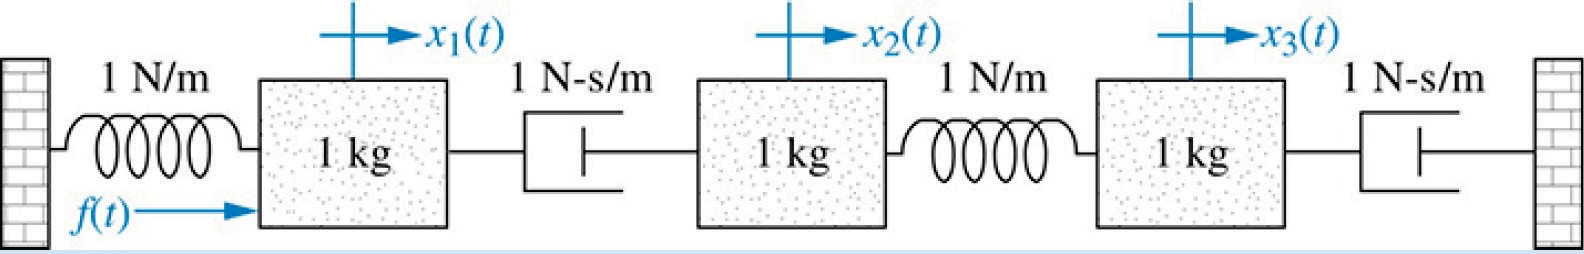
\includegraphics[width=\linewidth]{part01_translational_mechanical_system.png}
    \caption{Diagram of the translational mechanical system.}
    \label{fig:translational mechanical system}
\end{figure}

A state-space representation is a mathematical model of a physical system using variables that are in the time domain.

We are given the translational mechanical system
in Fig. \ref{fig:translational mechanical system}
that outputs $x_3\brao*t$.
From this system, let's define masses
\begin{equation}
    \vec{M} := \brac*{
        \begin{matrix} M_1 & M_2 & M_3 \end{matrix}
    }^\transpose = \brac*{
        \begin{matrix} \SI1{\kilo\gram} & \SI1{\kilo\gram} & \SI1{\kilo\gram} \end{matrix}
    }^\transpose\rlap,
\end{equation}
spring constants
\begin{equation}
    \vec{K} := \brac*{
        \begin{matrix} K_1 & K_2 \end{matrix}
    }^\transpose = \brac*{
        \begin{matrix} \SI1{\newton\per\meter} & \SI1{\newton\per\meter} \end{matrix}
    }^\transpose\rlap,
\end{equation}
and damping constants
\begin{equation}
    \vec{D} := \brac*{
        \begin{matrix} D_1 & D_2 \end{matrix}
    }^\transpose = \brac*{
        \begin{matrix} \SI1{\newton\second\per\meter} & \SI1{\newton\second\per\meter} \end{matrix}
    }^\transpose\rlap.
\end{equation}

\subsubsection{Free body diagram}
This system has the free body diagram shown in the CAD drawing on the following page.
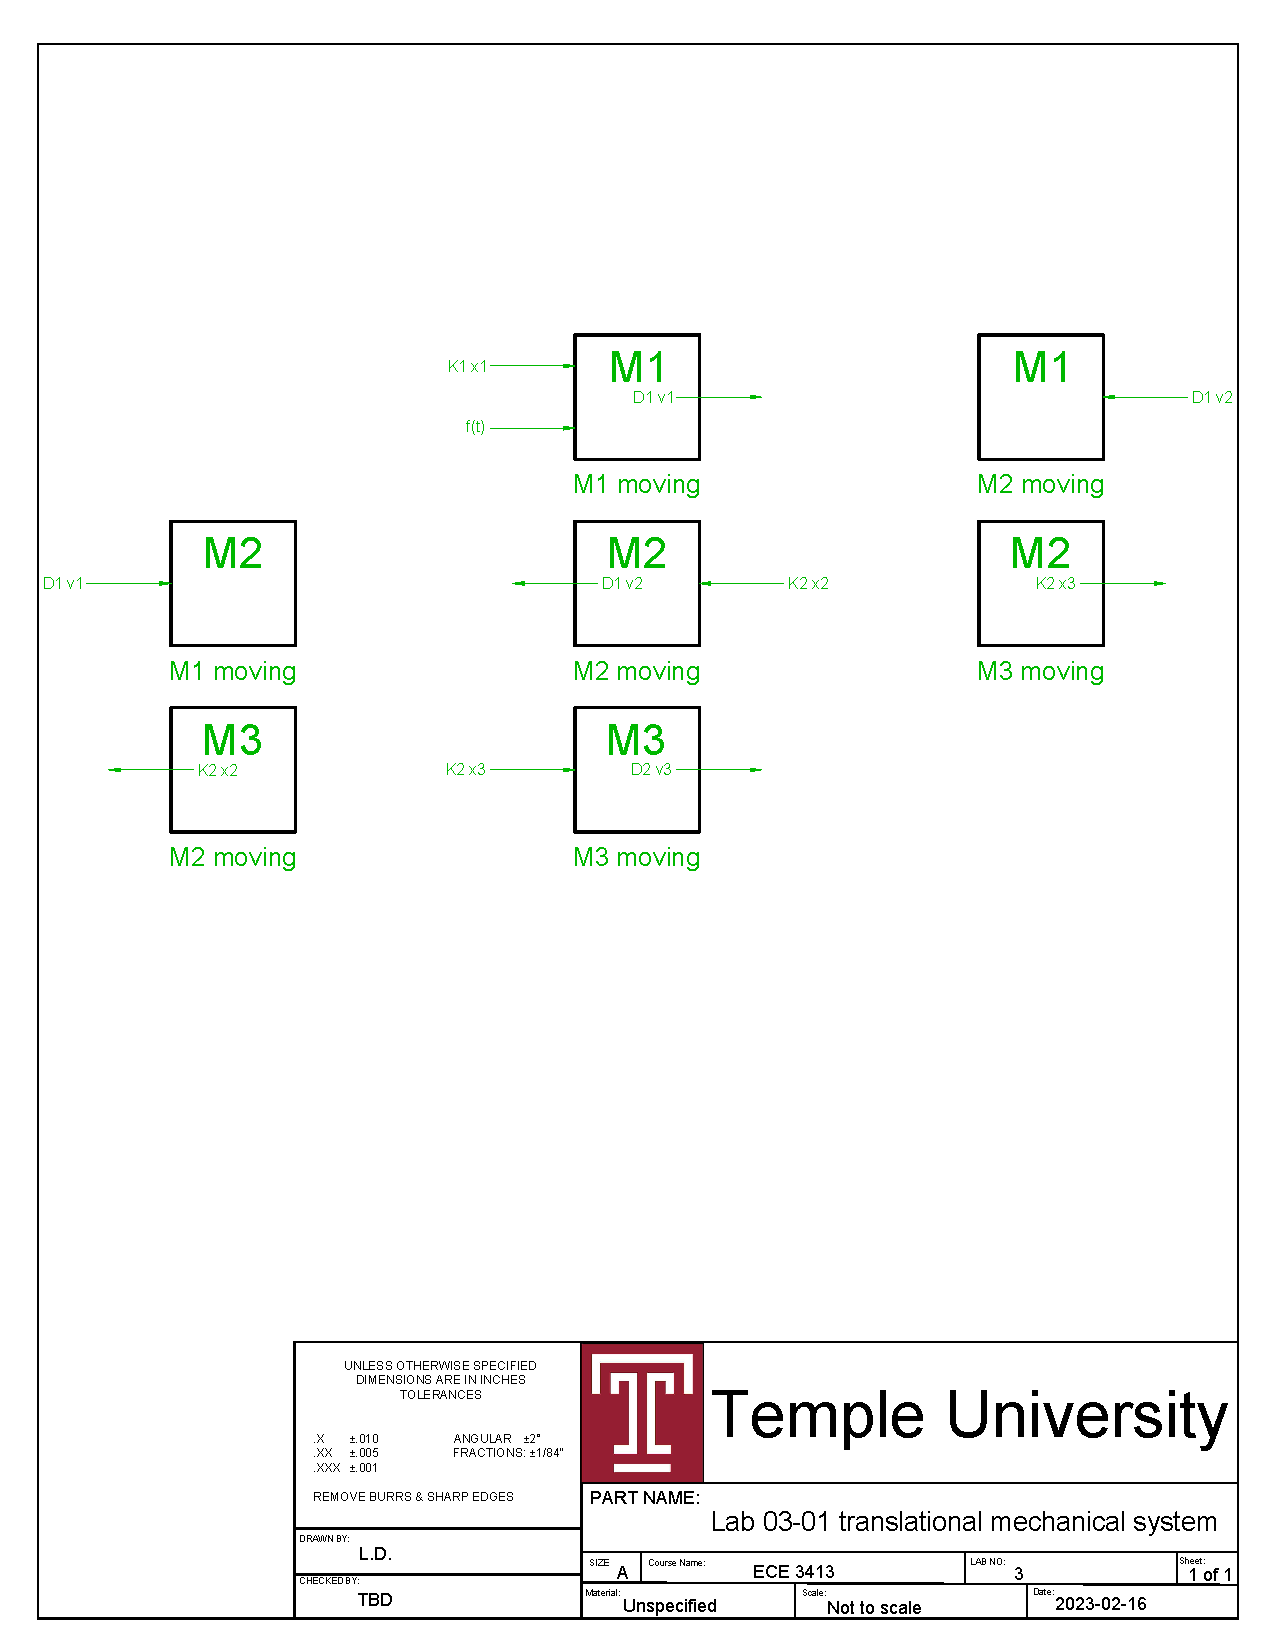
\includepdf{lab03-01 translational mechanical system fbd-A size.pdf}

\subsubsection{Mathematical state-space representation}

Then we find the total force at each mass applying superposition for each possible state.

\begin{equation}
    \piecefn*{
        \begin{array}{@{}l@{}}
            M_1 \ddot{x}_1 = \sum F_{M1\mathrm{x}} = K_1 x_1 + f\brao*t + D_1 \brao*{\dot{x}_1 - \dot{x}_2}\rlap,
        \\*
            M_2 \ddot{x}_2 = \sum F_{M2\mathrm{x}} = D_1\brao*{\dot{x}_1 - \dot{x}_2} + K_2\brao*{-x_2 + x_3}\rlap,
        \\*
            M_3 \ddot{x}_3 = \sum F_{M3\mathrm{x}} = K_2\brao*{-x_2 + x_3} + D_2\dot{x}_3\rlap.
        \\*
        \end{array}
    }
\end{equation}

Next, we relate states $\underline{\hat{x}} \in \mathbb{R}^6$ to position as in Table \ref{tab:states to position}.

\begin{table}[h]
    \centering
    \caption{How states relate to the position variables}
    \[
        \begin{array}{@{}r@{}c@{}l@{}}
        \toprule
            \text{state} & & \text{position}
        \\*
        \midrule
            {\hat{x}}_1 &{}={}& \dot{x}_1\rlap,
        \\*
            {\hat{x}}_2 &{}={}& x_1\rlap,
        \\*
            {\hat{x}}_3 &{}={}& \dot{x}_2\rlap,
        \\*
            {\hat{x}}_4 &{}={}& x_2\rlap,
        \\*
            {\hat{x}}_5 &{}={}& \dot{x}_3\rlap,
        \\*
            {\hat{x}}_6 &{}={}& x_3\rlap.
        \\*
        \bottomrule
        \end{array}
    \]
    \label{tab:states to position}
\end{table}

Thus, we can the derivatives of the states to the states with
the output $y := x_3 = {\hat{x}}_6$ represented by the first row
and using
the force equations for even rows, representing accelerations,
and the state--position relations for odd rows after the first, representing velocities,
giving the state-space representation

\begin{equation}
    \begin{array}{*4{@{}c}@{}}
            \mcadj1{@{}c@{}}{45}{}{\phantom{$=$}}{$
                = \brac*{
                    \begin{array}{@{}c@{}}
                        y
                    \\*
                    \midrule
                        \dot{\underline{\hat{x}}}
                    \\*
                    \end{array}
                }
            $}{}
        & &
            \mcadj1{@{}c@{}}{45}{}{\phantom{$=$}}{$
                =: \brac*{
                    \begin{array}{@{}c|c@{}}
                             D & \mathbf{C}
                    \\*
                    \midrule
                        \vec{B} & \mathbf{A}
                    \\*
                    \end{array}
                }
            $}{}
        &
            \mcadj1{@{}c@{}}{45}{}{\phantom{$=$}}{$
                = \brac*{
                    \begin{array}{@{}c@{}}
                        f
                    \\*
                    \midrule
                        \underline{\hat{x}}
                    \\*
                    \end{array}
                }
            $}{}
    \\*
        \brac*{
            \begin{array}{@{}c@{}}
                y \\*
            \midrule
                \dot{\hat{x}}_1 \\* \dot{\hat{x}}_2 \\*
                \dot{\hat{x}}_3 \\* \dot{\hat{x}}_4 \\*
                \dot{\hat{x}}_5 \\* \dot{\hat{x}}_6 \\*
            \end{array}
        }
        &{}={}&
        \brac*{
            \begin{array}{@{}c|*6c@{}}
                0 & 0 & 0 & 0 & 0 & 0 & 1
            \\*
            \midrule
                \sfrac1{M_1} & \sfrac{+D_1}{M_1} & \sfrac{K_1}{M_1} & \sfrac{-D_1}{M_1} & 0 & 0 & 0
            \\*
                0 & 1 & 0 & 0 & 0 & 0 & 0
            \\*
                0 & \sfrac{+D_1}{M_2} & 0 & \sfrac{-D_1}{M_2} & \sfrac{-K_2}{M_2} & 0 & \sfrac{+K_2}{M_2}
            \\*
                0 & 0 & 0 & 1 & 0 & 0 & 0
            \\*
                0 & 0 & 0 & 0 & \sfrac{-K_2}{M_3} &  \sfrac{D_2}{M_3} & \sfrac{+K_2}{M_3}
            \\*
                0 & 0 & 0 & 0 & 0 & 1 & 0
            \\*
            \end{array}
        }
        &
        \brac*{
            \begin{array}{@{}c@{}}
                f \\*
            \midrule
                {\hat{x}}_1 \\* {\hat{x}}_2 \\*
                {\hat{x}}_3 \\* {\hat{x}}_4 \\*
                {\hat{x}}_5 \\* {\hat{x}}_6 \\*
            \end{array}
        }.
    \end{array}
\end{equation}

\subsubsection{State-space representation in Matlab}

We can use the Matlab function \mintinline{matlab}{ss} to create a state-space representation object.
This function accepts the matrices of coefficients $\mathbf{A}$, $\vec{B}$, $\mathbf{C}$ and $D$ and returns a transfer function in state-space representation form.

This is a transfer function, just like the rational of polynomials \mintinline{matlab}{tf} and zero/pole/gain form \mintinline{matlab}{zpk}.
The $3$ types of objects are mutually convertible,
by using the target class's function on any transfer function object.

\subsection{Rational of polynomials form}

\subsubsection{Conversion using Matlab}

As stated in the previous section,
we may use the \mintinline{matlab}{tf} to convert from the state-space representation to the rational of polynomials form
just as we have with the zero/pole/gain form.
This gives us the transfer function
\begin{equation}
    T\brao*s = \brao*{\frac{x_3}{F}}\brao*s.
\end{equation}

\subsubsection{Equation for the transfer function}

Given a translational mechanical system with $m$ masses in movement,
we may find the transfer function using the equation
\begin{equation}
    T\brao*s = \mathbf{C}\brao*{s\mathbf{I}_{\brao*{2m}} - \mathbf{A}}\vec{B}
\end{equation}

We use Matlab to calculate the result and compare it to the converted transfer function.

\section{Results}

\hr

% This LaTeX was auto-generated from MATLAB code.
% To make changes, update the MATLAB code and export to LaTeX again.

\documentclass{article}

\usepackage[utf8]{inputenc}
\usepackage[T1]{fontenc}
\usepackage{lmodern}
\usepackage{graphicx}
\usepackage{color}
\usepackage{hyperref}
\usepackage{amsmath}
\usepackage{amsfonts}
\usepackage{epstopdf}
\usepackage[table]{xcolor}
\usepackage{matlab}

\sloppy
\epstopdfsetup{outdir=./}
\graphicspath{ {./part01_translational_mechanical_system_mlx_images/} }

\begin{document}

\matlabtitle{Part 1 $-$ Translational mechanical system}


\matlabheading{As a state-space model}

\begin{par}
\begin{flushleft}
is represented by the matrices of coefficients
\end{flushleft}
\end{par}

\begin{matlaboutput}
Mssr =
 
  A = 
       x1  x2  x3  x4  x5  x6
   x1   1   1  -1   0   0   0
   x2   1   0   0   0   0   0
   x3   1   0  -1  -1   0   1
   x4   0   0   1   0   0   0
   x5   0   0   0  -1   1   1
   x6   0   0   0   0   1   0
 
  B = 
       u1
   x1   1
   x2   0
   x3   0
   x4   0
   x5   0
   x6   0
 
  C = 
       x1  x2  x3  x4  x5  x6
   y1   0   0   0   0   0   1
 
  D = 
       u1
   y1   0
 
Continuous-time state-space model.
\end{matlaboutput}
\end{document}


\ \hr \\*

% This LaTeX was auto-generated from MATLAB code.
% To make changes, update the MATLAB code and export to LaTeX again.

\documentclass{article}

\usepackage[utf8]{inputenc}
\usepackage[T1]{fontenc}
\usepackage{lmodern}
\usepackage{graphicx}
\usepackage{color}
\usepackage{hyperref}
\usepackage{amsmath}
\usepackage{amsfonts}
\usepackage{epstopdf}
\usepackage[table]{xcolor}
\usepackage{matlab}

\sloppy
\epstopdfsetup{outdir=./}
\graphicspath{ {./part02_ratio_of_polynomials_form_mlx_images/} }

\begin{document}

\matlabtitle{Part 2 $-$ Rational of polynomials form}


\matlabheading{1. Conversion using Matlab}

\begin{par}
\begin{flushleft}
The transfer function from the state-space representation
\end{flushleft}
\end{par}

\begin{matlaboutput}
Mtf =
 
                   -s + 2.768e-16
  -------------------------------------------------
  s^6 - s^5 - s^4 - 2 s^3 + 2 s^2 + 2 s + 2.053e-16
 
Continuous-time transfer function.
\end{matlaboutput}

\matlabheading{2. Equation for transfer functions}

\begin{par}
\begin{flushleft}
create a transfer function that is just s
\end{flushleft}
\end{par}

\begin{matlaboutput}
T =
 
                   -s - 1.371e-16
  -------------------------------------------------
  s^6 - s^5 - s^4 - 2 s^3 + 2 s^2 + 2 s - 2.435e-16
 
Continuous-time transfer function.
\end{matlaboutput}

\matlabheading{Coefficient of determination $R^2$}

\begin{par}
\begin{flushleft}
To compare the transfer functions, let's find the $R^2$ value of all coefficients.
\end{flushleft}
\end{par}


\begin{par}
\begin{flushleft}
Then the R\textasciicircum{}2
\end{flushleft}
\end{par}

\begin{matlaboutput}
R2 = 1.0000
\end{matlaboutput}
\begin{matlaboutput}
shows that the coefficients have a strong correlation
\end{matlaboutput}
\begin{matlaboutput}
and are therefore equivalent.
\end{matlaboutput}
\end{document}


\section{Discussion}

After finding the state-space representation,
this experiment becomes very straightforward.
However, that is the difficult part.

What I remembered to help me finish it is that springs act on displacement into the moving mass and viscous dampers aft on velocity away from the moving mass.
After this, the sum of all forces must equal the acceleration of the mass.
Then setting up the matrix of coefficients is not difficult although I may not have been able to think of coming up with the variables myself.
It's a really clever way of solving this problem.

This experiment shows application not only in electrical engineering, but also mechanical and civil engineering of the concept of a control system.
It's interesting to imagine how many of the concepts that we have learned in electrical engineering may be applied to other engineering disciplines or may have even come from methods in other engineering disciplines.

Often times, it seems that less intuitive techniques may make a problem much easier to solve simply by changing the domain or a basis.
This is the principle behind using the Laplace transform to handle transfer functions more easily.

\newpage
\appendix
\section{Appendix}

\subsection{Part 1a -- Rise time, Matlab Script}\label{sap:solving for .9cf and .1cf}
\inputminted{matlab}{src/part01a_rise_time.m}

\end{document}
